\section{Cahier des charges}
Cette partie présente le cahier des charges du périphériques.
Elle intègre les quelques points fournis par le sujet auquel s'ajoutent les contraintes imaginées par les étudiants.
\hl{...}
\subsection{Objectif du circuit}
Le contrôleur d'interruptions a l pour rôle d'informer le processeur sur l’occurrence d'une interruption valide.
Il fournira alors l’adresse de la prochaine instruction à exécuter.

\subsection{Fonctionnalitées attendues}
Les fonctions de service du circuit sont :
\begin{enumerate}
    \item Masquer et démasquer chaque interruption individuellement
    \item Contenir le vecteur d'exception
    \item Etablir le niveau de priorité des interruptions
    \item Ne fournir au \gls{CPU} que les interruptions valides
    \item Prendre en compte les priorités dans la génération des demandes au \gls{CPU}
\end{enumerate}
\subsection{Utilisation du circuit}
	
Il s'agit ici de donner l'utilisation du circuit en présentant le schéma de câblage du contrôleur d'interruptions ainsi que la définition des signaux logiques d'entrées et sorties.
L'IP à concevoir s'interface avec le bus de données, le bus d'adresses ainsi qu'un ensemble de signaux de temporisation et de contrôle.
Il est possible de retrouver des signaux de temporisation comme le nWAIT et des signaux de contrôle comme le nRST ou le RnW.
Leur rôle est présenté table (\ref{tab:sens_role_signaux}).
	
\begin{figure}[H]
	\centering
	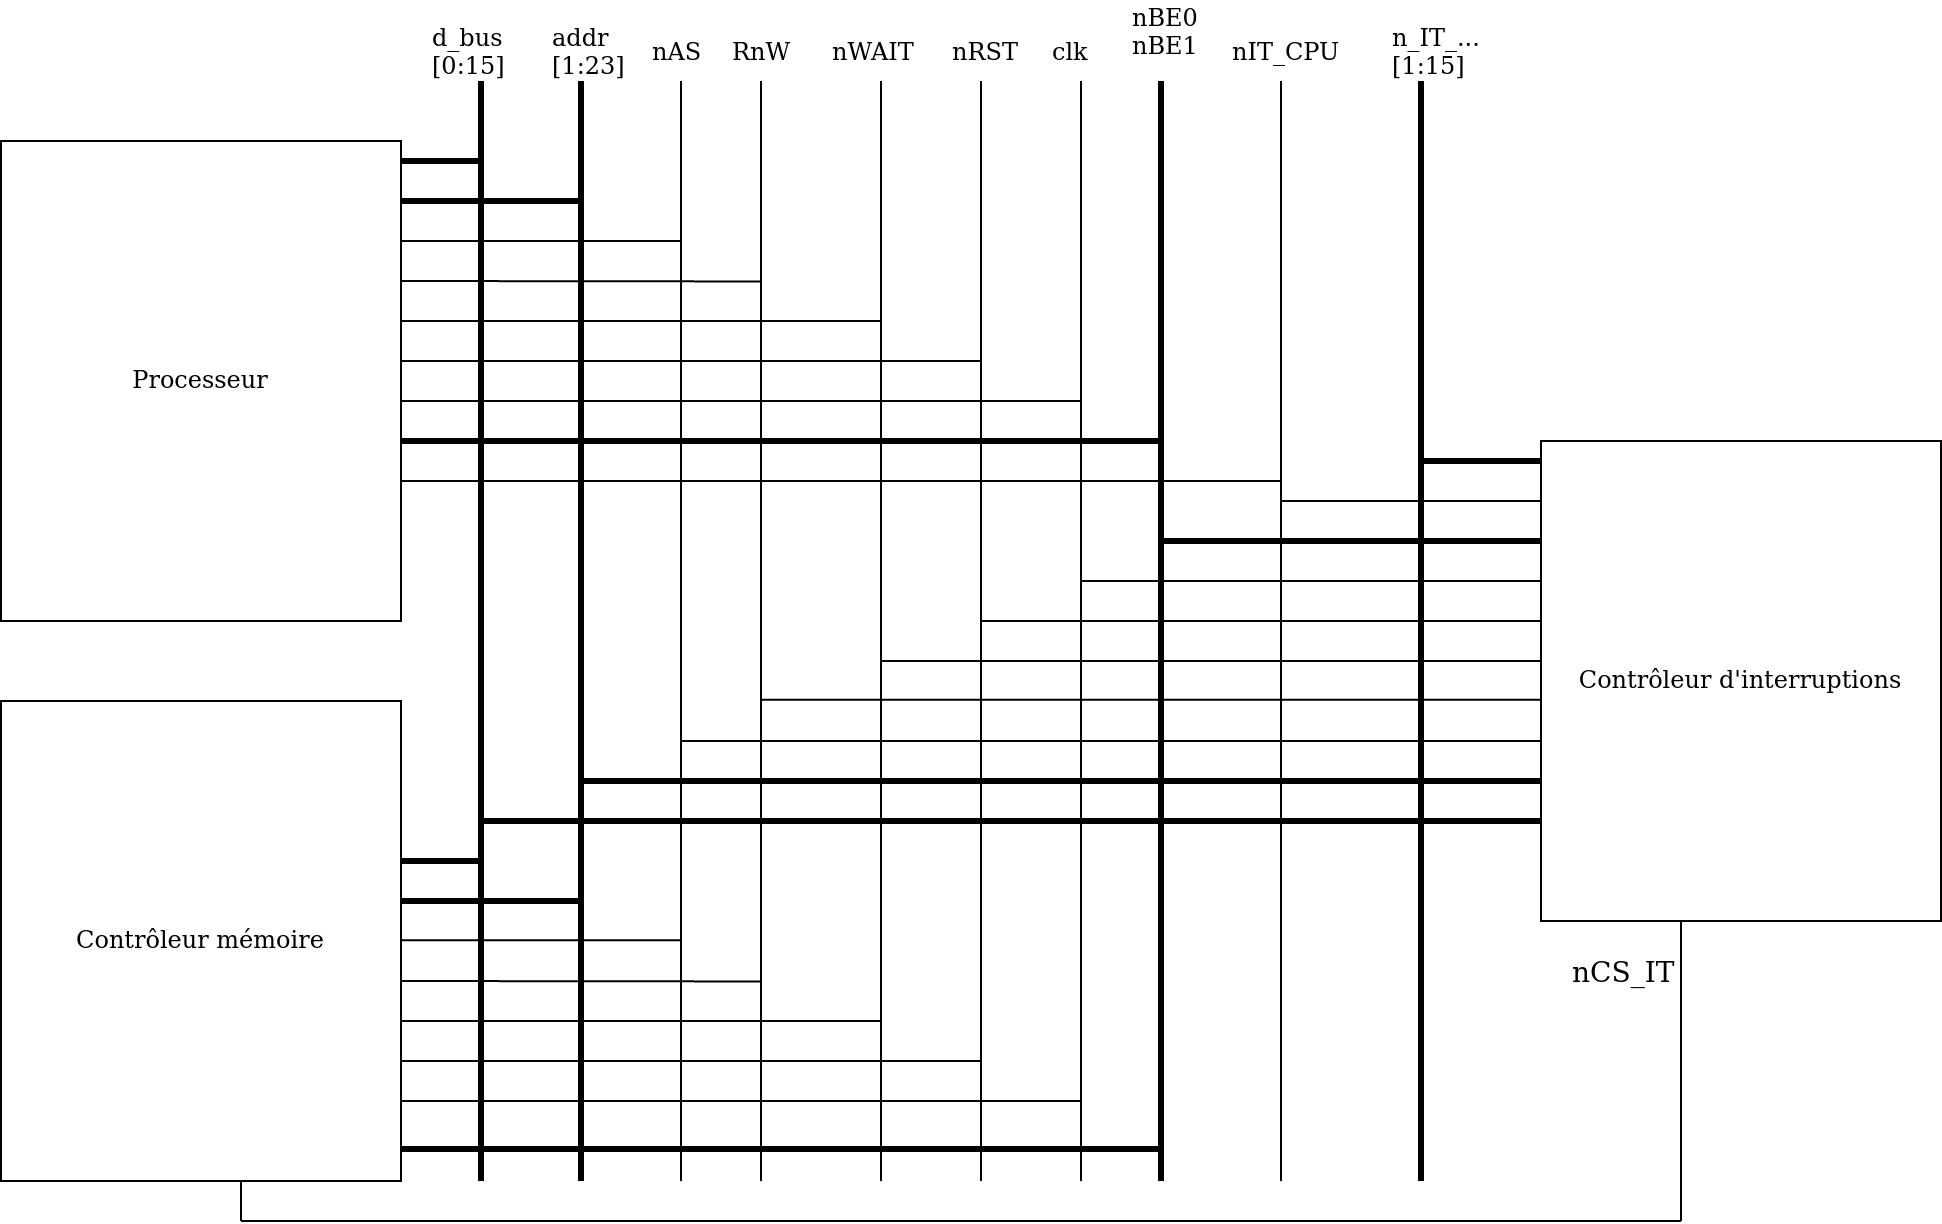
\includegraphics[width=1\linewidth]{figure/schema_cablage.png}
	\caption{Schéma de câblage de l'IP à concevoir, du contrôleur mémoire et du processeur}
	\label{fig:schema_cablage}
\end{figure}
	
Le contrôleur d'interruptions est également câblé avec plusieurs autres IPs du SoC.
Il y a par exemple le processeur avec lequel le signal nIT\_CPU est commun.
D'autre part le contrôleur mémoire est connecté avec le contrôleur d'interruptions par le signal nCS\_IT. L'ensemble des périphériques du SoC peut également envoyer un signal d'interruption représenté par nIT\_ $\dots$\\
	
Le schéma présenté ci-dessus ne précise pas le sens des signaux.
Il n'est donc pas possible de savoir quelles sont les entrées et sorties du contrôleur d'interruptions.
Également, les noms des 4 interruptions externes et des 11 autres provenant de divers périphériques ne sont pas donnés.
La figure et le tableau suivant présentent les entrées et sorties du point de vue de l'IP à concevoir ainsi que le rôle de chaque signaux. 
	
\begin{figure}[H]
	\centering
	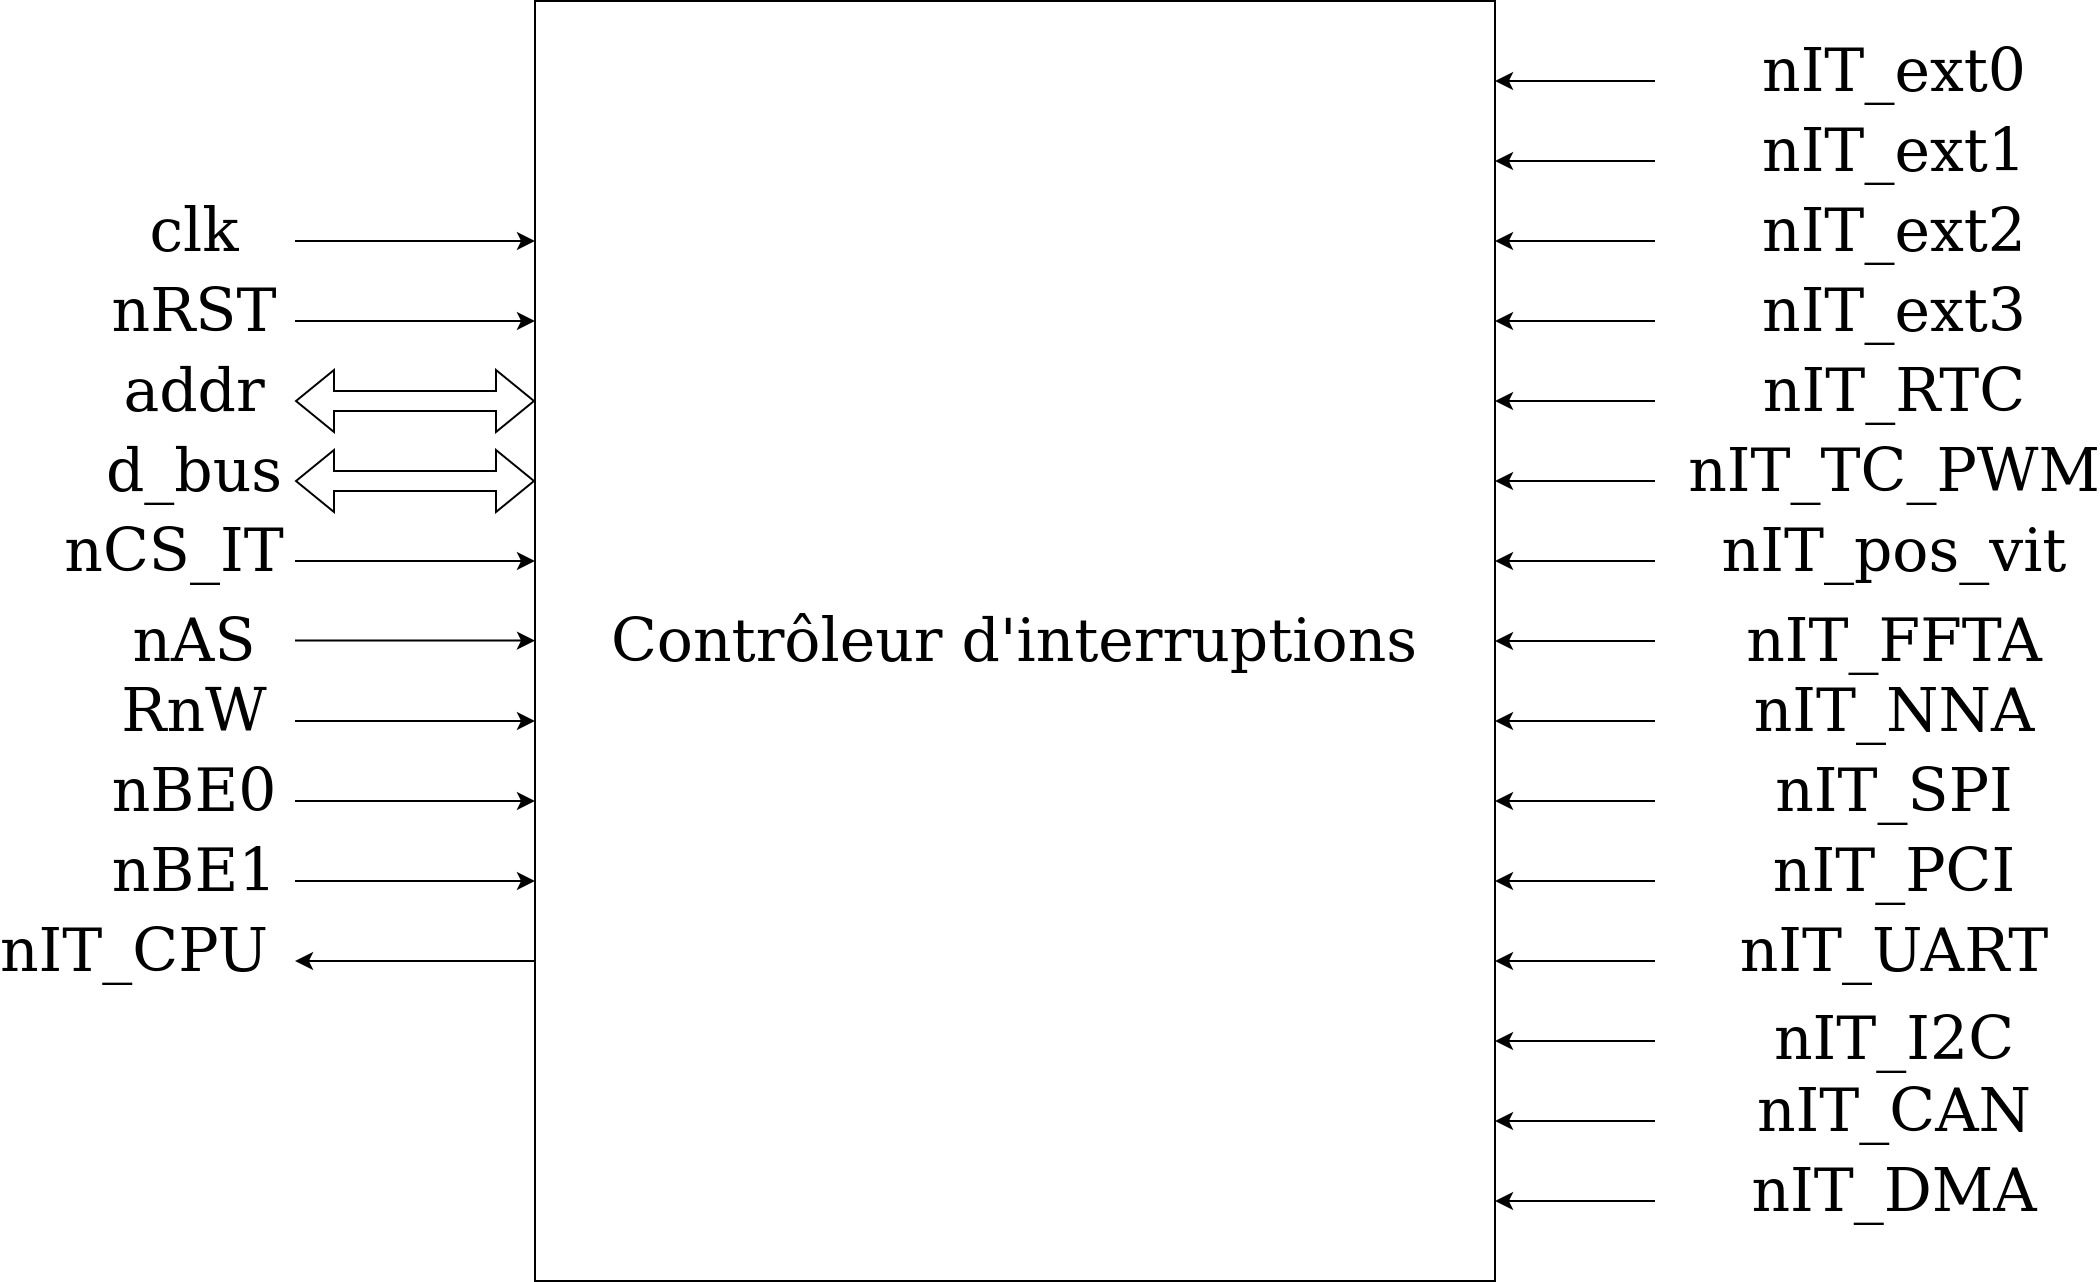
\includegraphics[width=1\linewidth]{figure/delimitation_systeme.png}
	\caption{Entrées et sorties de l'IP à concevoir}
	\label{fig:inout_ip}
\end{figure}	
	
\begin{table}[H]
	\centering
	\begin{tabular}{|c|c|c|}
		\hline
		Nom & Sens & Rôle\\
		\hline
		clk & Entrée & Signal d'horloge\\
		\hline
		nRST & Entrée & Signal de réinitialisation\\
		\hline
		addr & Entrée et sortie & Bus d'adresses\\
		\hline
		d\_bus & Entrée et sortie & Bus de données\\
		\hline
		nCS\_IT & Entrée & Signal de sélection du périphérique en cas \\
		& & de demande de lecture ou d'écriture\\
		\hline
		nAS & Entrée & Signal indiquant la présence d'une valeur sur le bus d'adresse\\
		\hline
		RnW & Entrée & Signal d'écriture ou de lecture\\
		\hline
		nBE0 & Entrée & \\
		\hline
		nBE1 & Entrée & \\
		\hline
		 &  & Signal pour le processeur avertissant \\
		nIT\_CPU & Sortie & qu'une interruption est demandée de la part d'un \\
		& & périphérique\\
		\hline
		nIT\_ext0 & Entrée & Signal d'interruption extérieure numéro 0\\
		\hline
		nIT\_ext1 & Entrée & Signal d'interruption extérieure numéro 1\\
		\hline
		nIT\_ext2 & Entrée & Signal d'interruption extérieure numéro 2\\
		\hline
		nIT\_ext3 & Entrée & Signal d'interruption extérieure numéro 3\\
		\hline
		nIT\_RTC & Entrée & Signal d'interruption provenant du périphérique RTC\\
		\hline
		nIT\_TC\_PWM & Entrée & Signal d'interruption provenant du Timer et PWM\\
		\hline
		nIT\_pos\_vit & Entrée & Signal d'interruption provenant du\\
		& & périphérique de mesure position et vitesse\\
		\hline
		nIT\_FFTA & Entrée & Signal d'interruption provenant de \\
		& & l'accélérateur transformée de Fourier discrète\\
		\hline
		nIT\_NNA & Entrée & Signal d'interruption provenant de \\
		& & l'accélérateur réseau de neurones\\
		\hline
		nIT\_SPI & Entrée & Signal d'interruption provenant du \\
		& & périphérique de communication SPI\\
		\hline
		nIT\_PCI & Entrée & Signal d'interruption provenant du \\
		& & périphérique de communication PCI\\
		\hline
		nIT\_UART & Entrée & Signal d'interruption provenant du \\
		& & périphérique de communication UART\\
		\hline
		nIT\_I2C & Entrée & Signal d'interruption provenant du \\
		& & périphérique de communication I2C\\
		\hline
		nIT\_CAN & Entrée & Signal d'interruption provenant du \\
		& & périphérique de communication CAN\\
		\hline
		nIT\_DMA & Entrée & Signal d'interruption provenant du \\
		& & périphérique d'accès direct à la mémoire.\\
		\hline
	\end{tabular}
	\caption{Sens et rôle des signaux}
	\label{tab:sens_role_signaux}
\end{table}
	
Il s'agit d'un signal envoyé au CPU pour lui signaler une interruption de la part d'un périphérique afin qu'il arrête les tâches en cours et qu'il lise sur le bus de données l'adresse de la routine d'interruption à laquelle il doit brancher.


\subsection{Chronogrammes caractéristiques}

\subsection{Contraintes du projet}

